\documentclass[a4paper,12pt]{article}

% Paquetes necesarios
\usepackage[utf8]{inputenc}   % Codificación de caracteres UTF-8
\usepackage[catalan]{babel}    % Idioma catala
\usepackage{geometry}         % Configuración de márgenes
\geometry{left=3cm,right=2.5cm,top=2.5cm,bottom=3cm}
\usepackage{fancyhdr}         % Cabeceras y pies de página personalizados
\usepackage{parskip}          % Evita indentación en los párrafos
\usepackage{graphicx}
\usepackage{minted}
\usepackage{subcaption}
\usepackage{tikz}
\usepackage{amsmath}
\usepackage{amsthm}

\usepackage{enumitem}

\usepackage{booktabs}
\usepackage{todonotes}

\DeclareRobustCommand{\bigO}{%
  \text{\usefont{OMS}{cmsy}{m}{n}O}%
}

% Personalización de cabeceras
\pagestyle{fancy}
\fancyhf{}
\fancyhead[L]{Problemes algorísimia}
\fancyhead[R]{Grup G11.2}

\fancyfoot[C]{\thepage}

% Configuración de título
\title{Problemes algorísimia}
\author{Miquel Pere Baztán Grau
    \\ Bernat Dosrius Lleonart
    \\ Xavier Momplet Gil
    \\ Emma Ventura Font 
    \\ \\   Universitat Politècnica de Catalunya}
\date{21 de desembre 2024}

\begin{document}

\maketitle

\section*{Setmana 2 (20 febrer)}

\subsection*{Problema 1.3 (celebritat?)}
\textbf{En una festa, un convidat es diu que és una celebritat si tothom el coneix, però ell no coneix a ningú (tret d'ell mateix). Les relacions de coneixença donen lloc a un graf dirigit: cada convidat és un vèrtex, i hi ha un arc entre $u$ i $v$ si $u$ coneix a $v$.}

\begin{enumerate}[label=(\alph*)]
    \item \textbf{Doneu una formalització de la propietat de ser celebritat.} \\ \\
    Sigui $G = (V,E)$ un graf dirigit. Una celebritat és un vèrtex $$v \in V \ | \ \forall v' \in V \ v' \neq v \ \Longrightarrow \ (v', v) \in E \ i \ (v, v') \notin E$$
    \item \textbf{Doneu un algorisme que, donat un graf dirigit representat amb una matriu d'adjacència, indica si hi ha o no cap celebritat. En el cas que hi sigui, cal dir qui és. El vostre algorisme ha de funcionar en temps $\bigO(n)$, on $n$ és el nombre de vèrtexs.} \\ \\
    Notem que, per la definició de celebritat, només pot existir una celebritat donat un graf dirigit simple. També cal notar que la matriu amb la que treballarem en aquest problema és una matriu que només té $1's$ i $0's$ a les seves entrades. \\
    Sigui $a_{ij}$ l'entrada de la i-èssima fila i la j-èssima columna de la matriu d'adjacència, aleshores:
    $$a_{ij} = \begin{cases}
        0 \ &$si$ \ (i,j)  \in E \\
        1 \ &$si$ \ (i,j) \notin E
    \end{cases} $$
    Per a determinar si el graf té una celebritat, començarem des de la posició $(0,0)$ de la matriu, anem augmentant $j$ fins a trobar un $1$, això ens indica que el vèrtex de la fila en la que ens trobem no és famós (ja que coneix a un altre vèrtex). Un cop trobat aquest $1$ saltem a la fila $j$ ($i = j$) i seguim agumentant $j$ fins a trobar un $1$ o fins a arribar a $j == n$. En el moment en que $j == n$, tenim un candidat a celebritat (i-èssim vèrtex). Per a comprovar si $i$ és una celebritat cal recòrrer la i-èssima fila i la j-èssima columna, cal comprovar:
    $$\forall \ k \in [n-1] \ | \ k \neq i \ a_{kj} == 1$$
    $$\forall \ l \in [n-1] \ a_{il} == 0$$
    Aquestes dues condicions ens diuen que el vèrtex $i$ és conegut per tots els altres vèrtex i ell mateix no coneix a cap altre vèrtex i, per tant, és una celebritat. Si no es verifiquen les dues condicions anteriors quan $j==n$, aleshores no existeix cap celebritat en G. 
    \end{enumerate}

\subsection*{Problema 1.9 (és fortament connex?)}
\textbf{Un graf dirigit és fortament connex quan, per cada parell de vèrtexs $u$, $v$, hi ha un camí de $u$ a $v$. Doneu un algorisme per determinar si un graf dirigit és fortament connex.} \\ \\
Sigui $R$ una relació d'equivalència  



\subsection*{Problema 1.10 (és semiconnex?)}
Un graf dirigit $G = (V, E)$ és semiconnex si, per qualsevol parell de vèrtexs $u, v \in V$, tenim un camí dirigit de $u$ a $v$ o de $v$ a $u$.
Doneu un algorisme eficient per determinar si un graf dirigit $G$ és semiconnex. Demostreu la correctesa del vostre algorisme i analitzeu-ne el cost. Dissenyeu el vostre algorisme fent us d'un algorisme que us proporcioni les components connexes fortes del graf en temps $\bigO(n + m)$.

\newpage
\subsection*{Problema 1.12 (clique max?)}
Donat un graf no dirigit $G = (V, E)$ i un subconjunt de vèrtex V1, el subgraf
induït per $V1$, $G[V1]$ té com a vèrtex $V1$ i con a arestes totes les arestes a $E$ que connecten
vèrtexs en $V1$. Un clique és un subgraf indiut per un conjunt $C$ on tots els vèrtexs estan
connectats entre ells.
Considereu el següent algorisme de dividir-i-vèncer per al problema de trobar un clique en un
graf no dirigit $G = (V, A)$.
\begin{figure}[H]
    \centering
    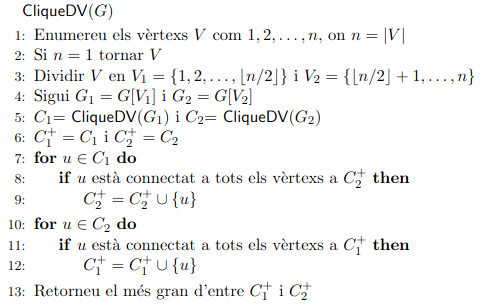
\includegraphics[width=0.8\linewidth]{ksnip_20250219-180045.png}
    \caption{Enter Caption}
    \label{fig:enter-label}
\end{figure}
Contesteu les següents preguntes:
\begin{enumerate}[label=(\alph*)]
    \item Demostreu que l’algorisme CliqueDV sempre retorna un subgraf de G que és un clique.
    \item Doneu una expressió asimptòtica del nombre de passos de l’algorisme CliqueDV.
    \item Doneu un exemple d’un graf G on l’algorisme CliqueDV retorna un clique que no és de
grandària màxima.
    \item Creieu que és fàcil modificar CliqueDV de manera que sempre done el clique màxim,
sense incrementar el temps pitjor de l’algorisme? Expliqueu la vostra resposta
\end{enumerate}



\todo[inline]{Assignació setmana 2 (20 febrer):
1.3, 1.9, 1.10, 1.12
Extra 1: Definiu formalment la propietat connex(G) que descriu si un graf G=(V,E) és connex.
Extra 2: Definiu formalment la propietat clique(G) que descriu si un graf G=(V,E) és complet.
Extra 3: Sigui B(n) el nombre de fulles en un arbre binari complet amb n nodes. Demostreu mitjançant inducció que: B(n)= n+1 / 2, per tot n ≥1.
(per a tots els grups)}














\newpage

$$$$

\vfill

\begin{center}
    \rule{0.8\textwidth}{0.5pt} % Línia separadora subtil

    \vspace{.5cm}
    
    % Dibuix abstracte amb corbes i arcs
    \begin{tikzpicture}
        % Curva principal amb un gradient subtil
        \draw[thick, color=blue!60!white] plot [smooth cycle, tension=1] coordinates {(0,0) (2,0.5) (3,-0.2) (4,0.6) (6,0)};
        
        % Segona corba més subtil
        \draw[thick, color=blue!30!white] plot [smooth, tension=1] coordinates {(0.5,-0.5) (2,0.2) (3,-0.3) (5,0.4) (6.5,0)};
        
        % Tercera corba lleugerament separada
        \draw[thick, color=blue!10!white] plot [smooth, tension=1] coordinates {(1,-1) (2.5,0.1) (3,-0.5) (5.5,0.3) (7,0)};
        
        % Petits cercles decoratius al final de les corbes

    \end{tikzpicture}

    \textbf{Miquel Pere Baztán Grau\\ Bernat Dosrius Lleonart
    \\ Xavier Momplet Gil
    \\ Emma Ventura Font} \\% Nom de l'estudiant
    \vspace{0.2cm}
    Universitat Politècnica de Catalunya \\ % Nom de la institució
    \vspace{0.5cm}
    \rule{0.4\textwidth}{0.4pt} % Línia final subtil
\end{center}

\vfill

\end{document}
